\documentclass[12pt]{article}

\usepackage{amsmath}
\usepackage{amsfonts}
\usepackage{graphicx}

\author{Andrew Mason}
\title{EECS 440 HW2}

\begin{document}
\maketitle

\begin{enumerate}
  \item Suppose $f$ and $g$ are two convex functions defined on
  $\mathbb{R}^n$.
  \begin{enumerate}
    \item Show that $h = f + g$ is also convex.\\

    For $h$ to be convex, we need to have that:\\
    $h(\lambda x_1 + (1 - \lambda)x_2) \leq
      \lambda h(x_1) + (1 - \lambda)h(x_2)$\\
    Since $h = f + g$, we can expand both sides and get:\\
    $f(\lambda x_1 + (1 - \lambda)x_2) + g(\lambda x_1 + (1 - \lambda)x_2)
      \leq\lambda f(x_1) + (1 - \lambda)f(x_2) +
      \lambda g(x_1) + (1 - \lambda)g(x_2)$\\
    Now, $f$ and $g$ are both convex, so we know that
      $f(\lambda x_1 + (1 - \lambda)x_2)\leq
      \lambda f(x_1) + (1 - \lambda)f(x_2)$ and
      $g(\lambda x_1 + (1 - \lambda)x_2)\leq
      \lambda g(x_1) + (1 - \lambda)g(x_2)$\\
    From this, the original inequality holds, so $h$ is convex.
    \item Show that $h = max(f, g)$ is also convex.\\

    For $h$ to be convex, we need to have that:\\
    $h(\lambda x_1 + (1 - \lambda)x_2) \leq
      \lambda h(x_1) + (1 - \lambda)h(x_2)$\\
    Without loss of generality, let $max(
      f(\lambda x_1 + (1 - \lambda)x_2),
      g(\lambda x_1 + (1 - \lambda)x_2) =
      f(\lambda x_1 + (1 - \lambda)x_2))$\\
    Now, we need $f(\lambda x_1 + (1 - \lambda)x_2)\leq
      \lambda max(f(x_1), g(x_1)) + (1 - \lambda)max(f(x_2), g(x_2))$\\
    In the case that $f(x_1)\geq g(x_1)$ and $f(x_2)\geq g(x_2)$, we know
      that $h$ is convex, since $h = f$.\\
    In the case that $f(x_1) < g(x_1)$ or $f(x_2) < g(x_2)$, then $h$ is
      still convex, since $\lambda h(x_1) + (1 - \lambda)h(x_2)$ is
      strictly greater than $\lambda f(x_1) + (1 - \lambda)f(x_2)$.
    \item Show whether $h = f - g$ is convex or not.\\

    $h$ is not convex.\\
    Let $f(x) = x^2$ and $g(x) = 2x^2$.\\
    Then $h(x) = -x^2$.\\\\
    Now, let $x_1 = -1$, $x_2 = 1$, $\lambda = \frac{1}{2}$.\\
    $h(\lambda x_1 + (1 - \lambda)x_2) \leq
      \lambda h(x_1) + (1 - \lambda)h(x_2)$\\
    $h(-\frac{1}{2} + \frac{1}{2}) \leq
      \frac{1}{2}h(-1) + \frac{1}{2}h(1)$\\
    $0 \leq -\frac{1}{2} - \frac{1}{2}$\\
    $0 \leq -1$\\
  \end{enumerate}

  \item Show that the set $C=\{x|Ax \geq b\}$, $A \in \mathbb{R}^{m\times n}$
    , $x \in \mathbb{R}^n$, $b \in \mathbb{R}^m$ is a convex set. Note
    that this describes the constraint set of a linear program.

    Let $x_1, x_2\in C$.\\
    Define $x = \lambda x_1 + (1 - \lambda)x_2$.\\
    Need to show that $Ax\geq b$\\
    $A(\lambda x_1 + (1-\lambda)x_2) =
      \lambda Ax_1 + (1-\lambda)Ax_2\geq
      \lambda b + (1-\lambda)b =
      b(\lambda + 1 - \lambda) = b$\\

  \item Consider the primal linear program
    min $c^Tx$ s.t. $Ax\geq b, x\geq 0$
    And its dual
    max $b^Tu$ s.t. $A^Tu\leq c, u\geq 0$.
    Carefully prove that for any feasible $(x, u)$, $b^Tu\leq c^Tx$\\

    First, work with the dual: $A^Tu\leq c$\\ Multiplying by $x$, we get
    $x^TA^Tu\leq x^Tc$\\
    Taking the transpose of both sides yields $u^TAx\leq c^Tx$\\
    Similarly, with the primal, we have $Ax\geq b$\\
    Multiplying by $u$ we get $u^TAx\geq u^Tb$\\
    Now, we see that $u^Tb\leq u^TAx\leq c^Tx$
  \item Prove that the set of all continuous probability distributions over
    [0, 1] is convex.\\

    Let $S$ be the set of continuous probability distributions over [0,1].\\
    Let $f, g\in S$.\\
    Then $h = \lambda f + (1-\lambda)g \in S$\\
    $h$ is continuous because it is the sum of two continuous functions.\\
    Also, $h$ is non-negative $\forall e\in\Omega$, since $f,g$ are both non-negative.\\
    Finally, we need $\int_{-\infty}^{\infty} h(x) dx = 1$.\\\\

    $\int_{-\infty}^{\infty} h(x) dx =$
      $\int_{-\infty}^{\infty} \lambda f(x) + (1 - \lambda) g(x) dx$\\
    $\int_{-\infty}^{\infty} h(x) dx =$
      $\int_{-\infty}^{\infty} \lambda f(x) dx + \int_{-\infty}^{\infty} (1-\lambda)g(x) dx$\\
    $\int_{-\infty}^{\infty} h(x) dx =$
      $\lambda + 1 - \lambda$\\
    $\int_{-\infty}^{\infty} h(x) dx = 1$\\

    So $h\in S$ and $S$ is convex.
  \item Consider the LP:
  \begin{enumerate}
    \item Draw the feasible region in $\mathbb{R}^2$.\\\\
    See Figure 1 below.
    \item Draw the contours of $c^Tx = -12$, $c^Tx = -14$ and $c^Tx = -16$
      and determine the solution graphically.\\\\
    See Figure 2 below. The graphical solution is $x_1 = 4$, $x_2 = 5$.
    \item Solve the problem using the simplex method. On your figure, trace
      the path taken by the simplex method as it moves to the solution.\\\\
      See Figure 3 below. The simplex solution is $x_1 = 4$, $x_2 = 5$.
  \end{enumerate}
  \begin{figure}
    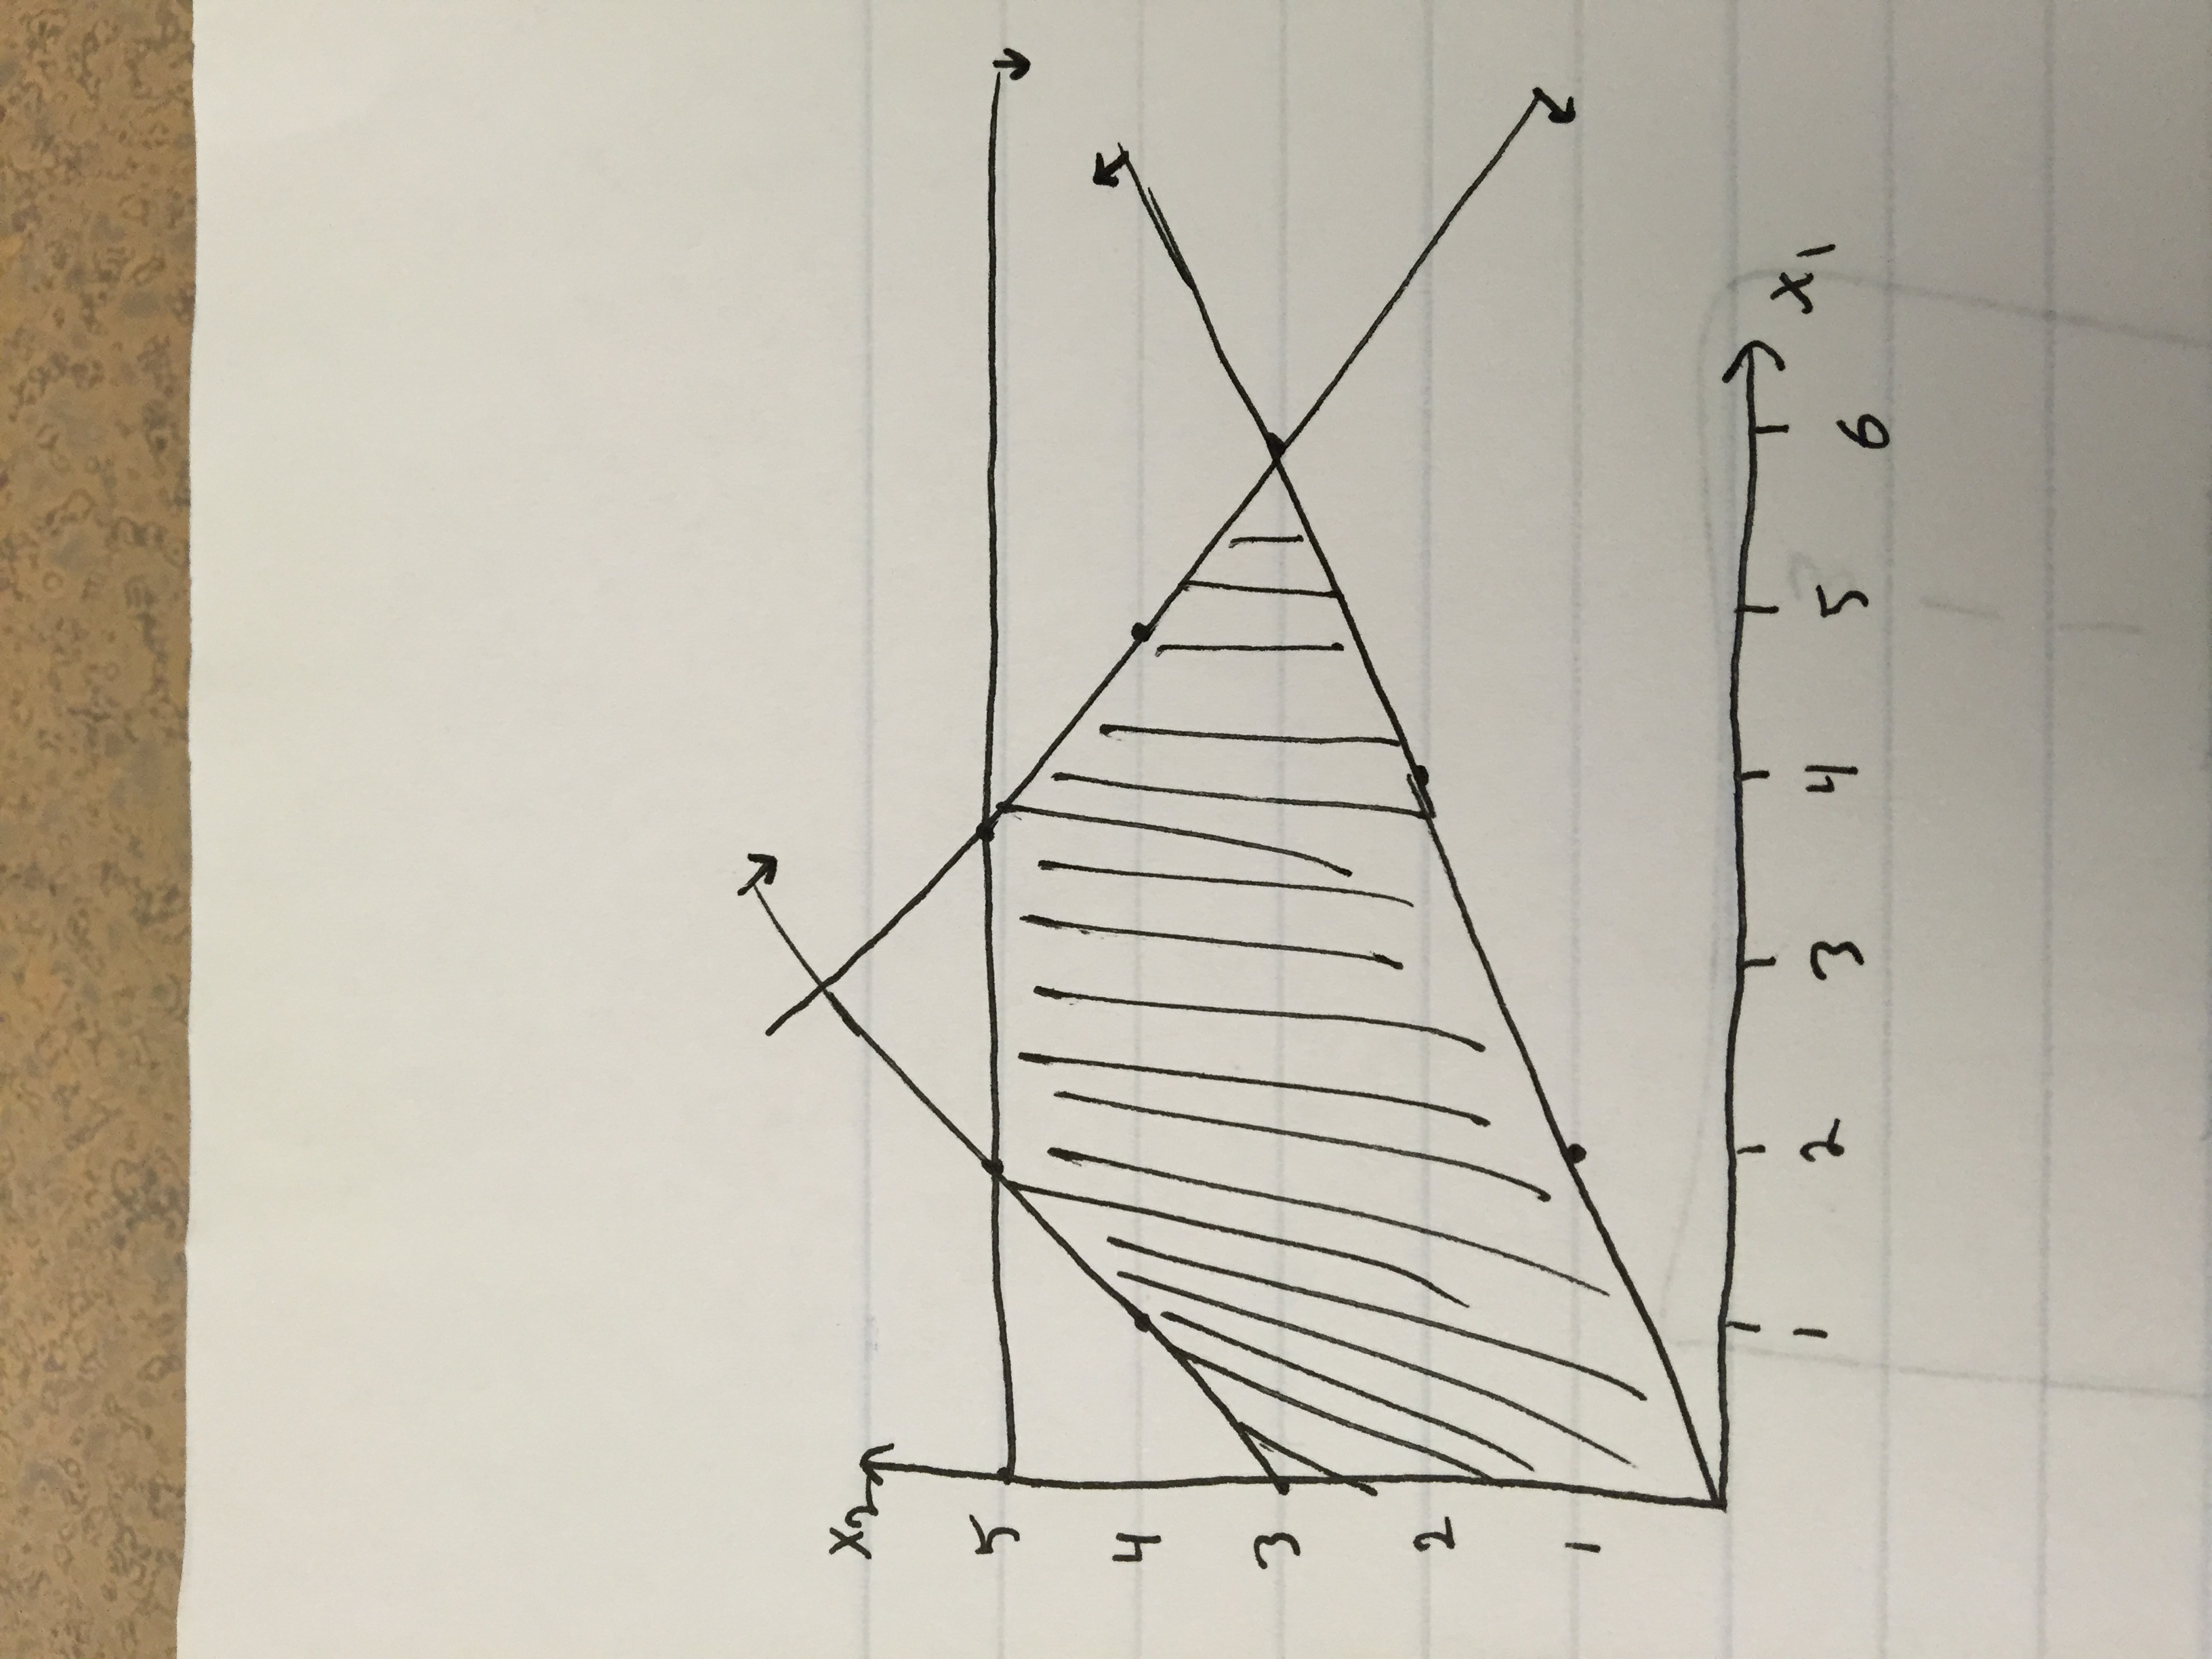
\includegraphics[width=\linewidth,angle=-90]{feasible_region.jpg}
    \caption{Feasible region of the linear program}
  \end{figure}
  \begin{figure}
    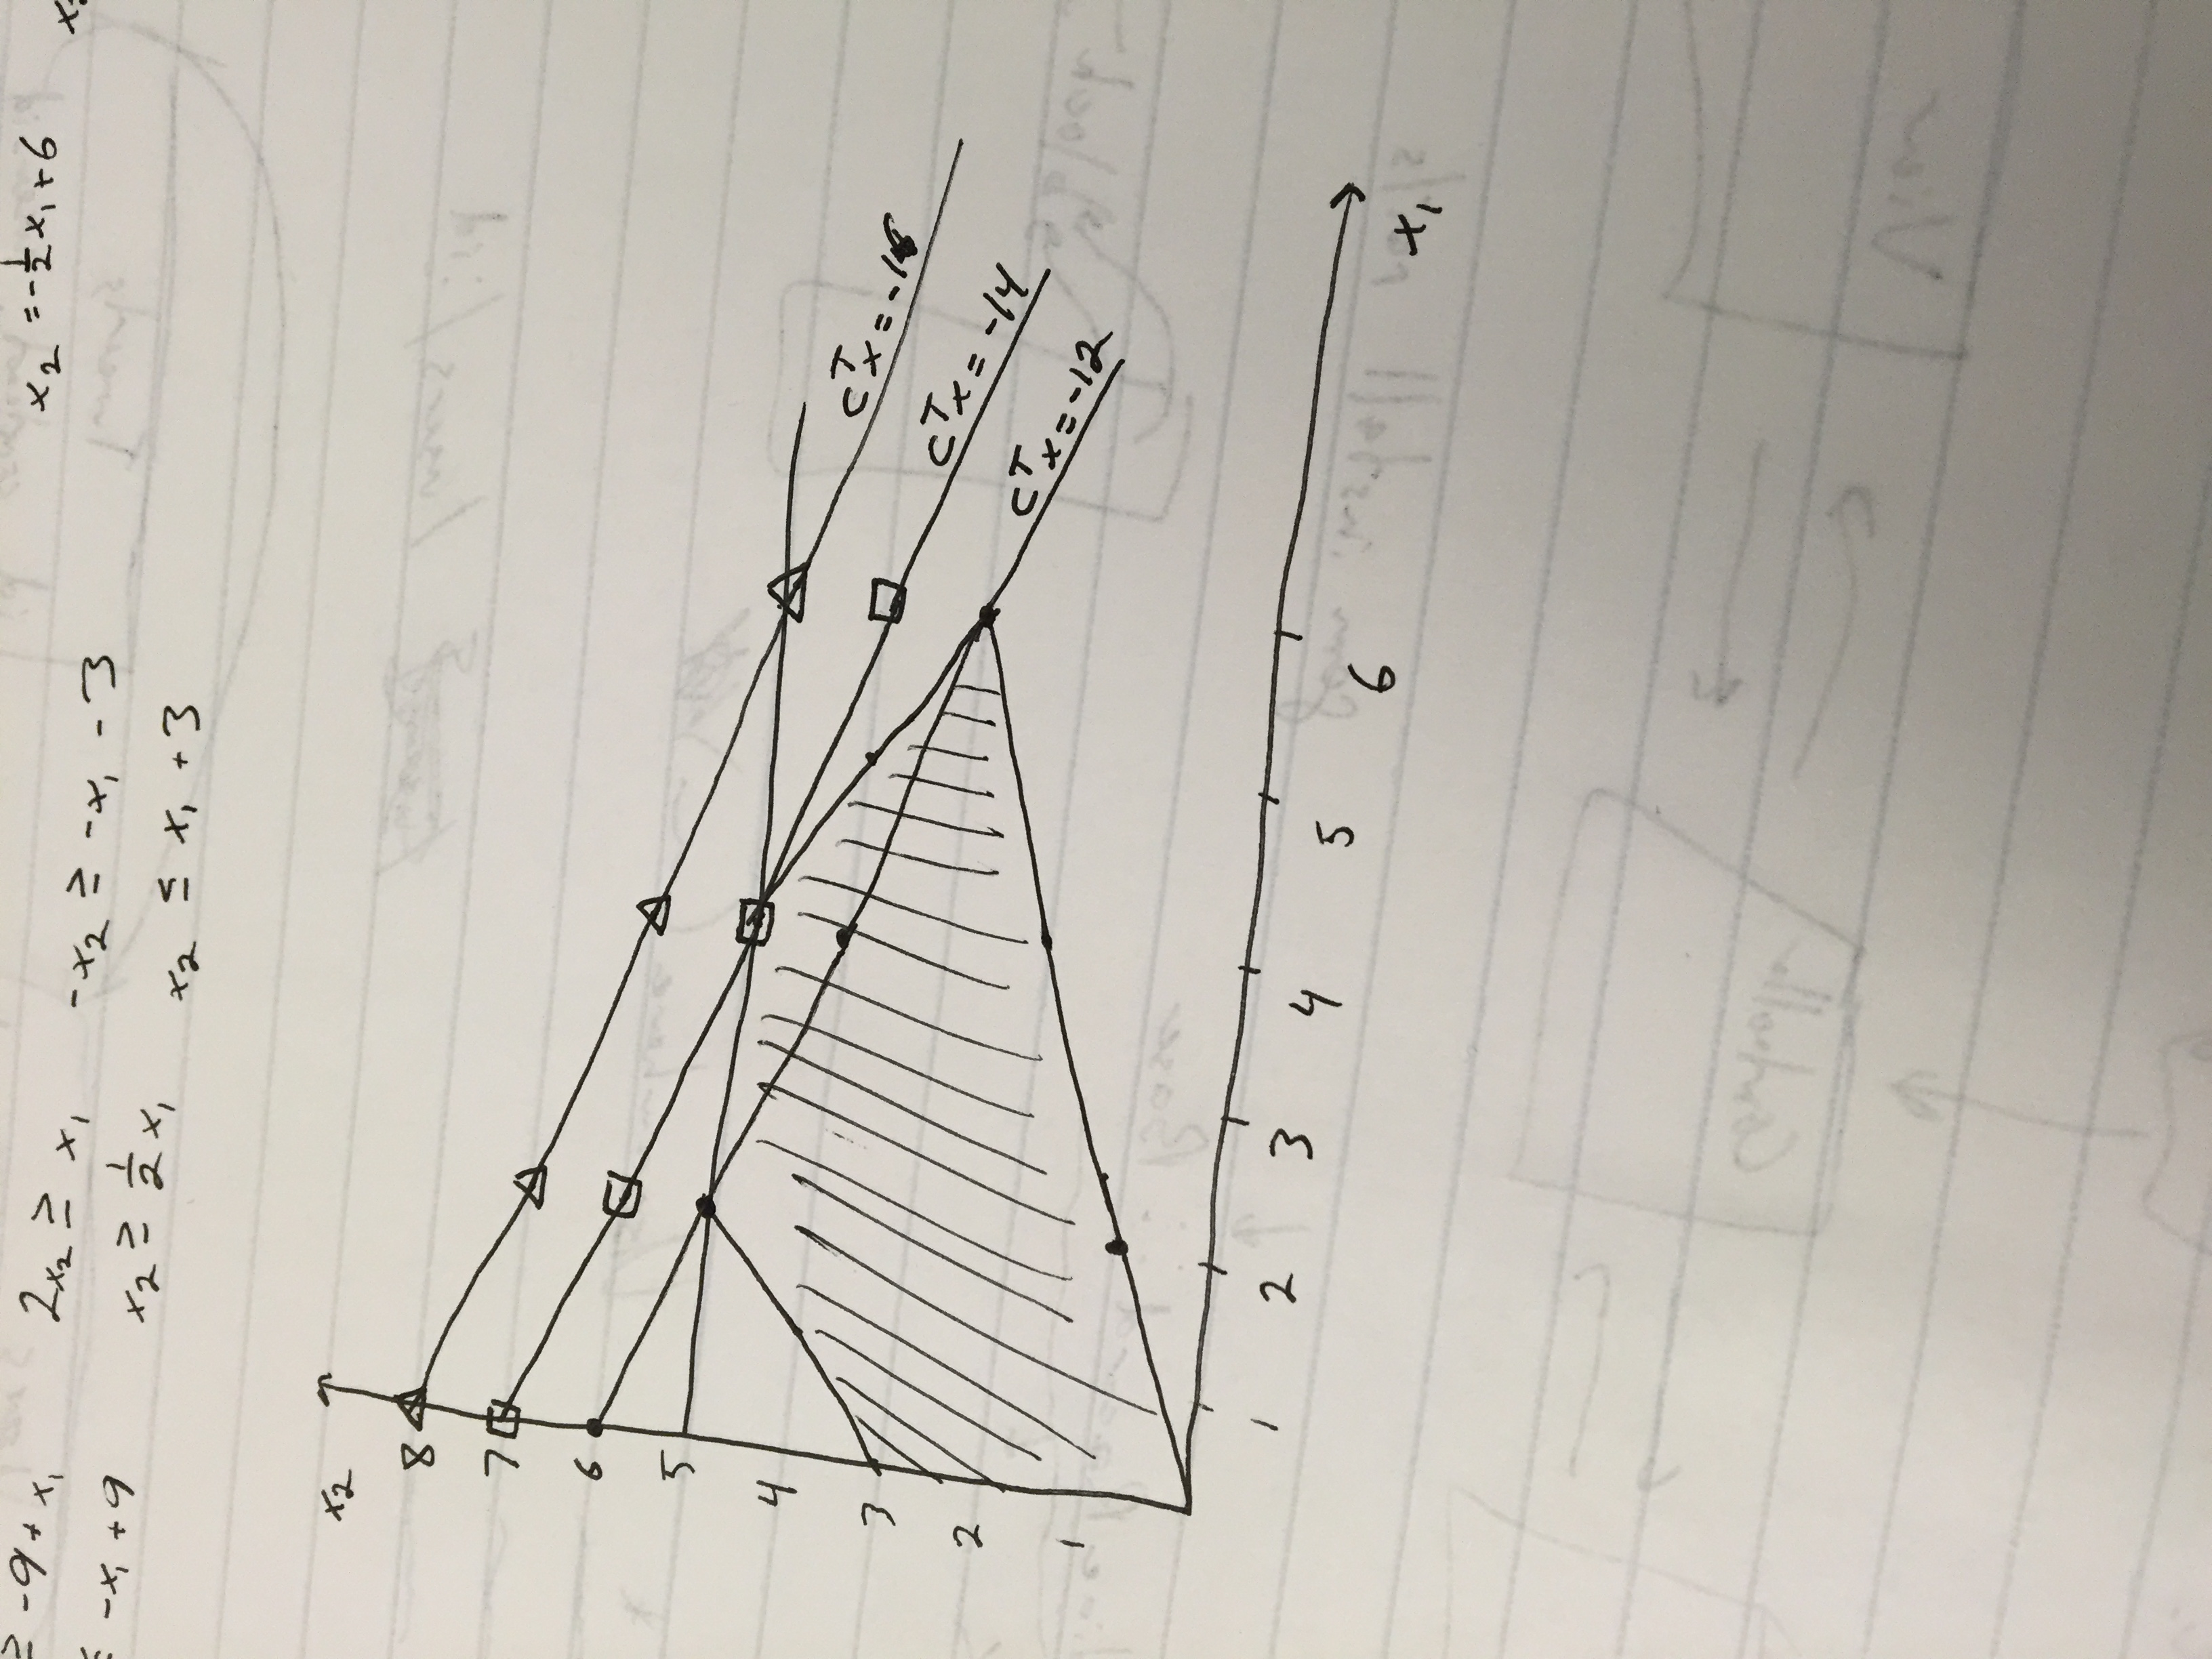
\includegraphics[width=\linewidth,angle=-90]{contours.jpg}
    \caption{Contours of $c^Tx = {-12, -14, -16}$}
  \end{figure}
  \begin{figure}
    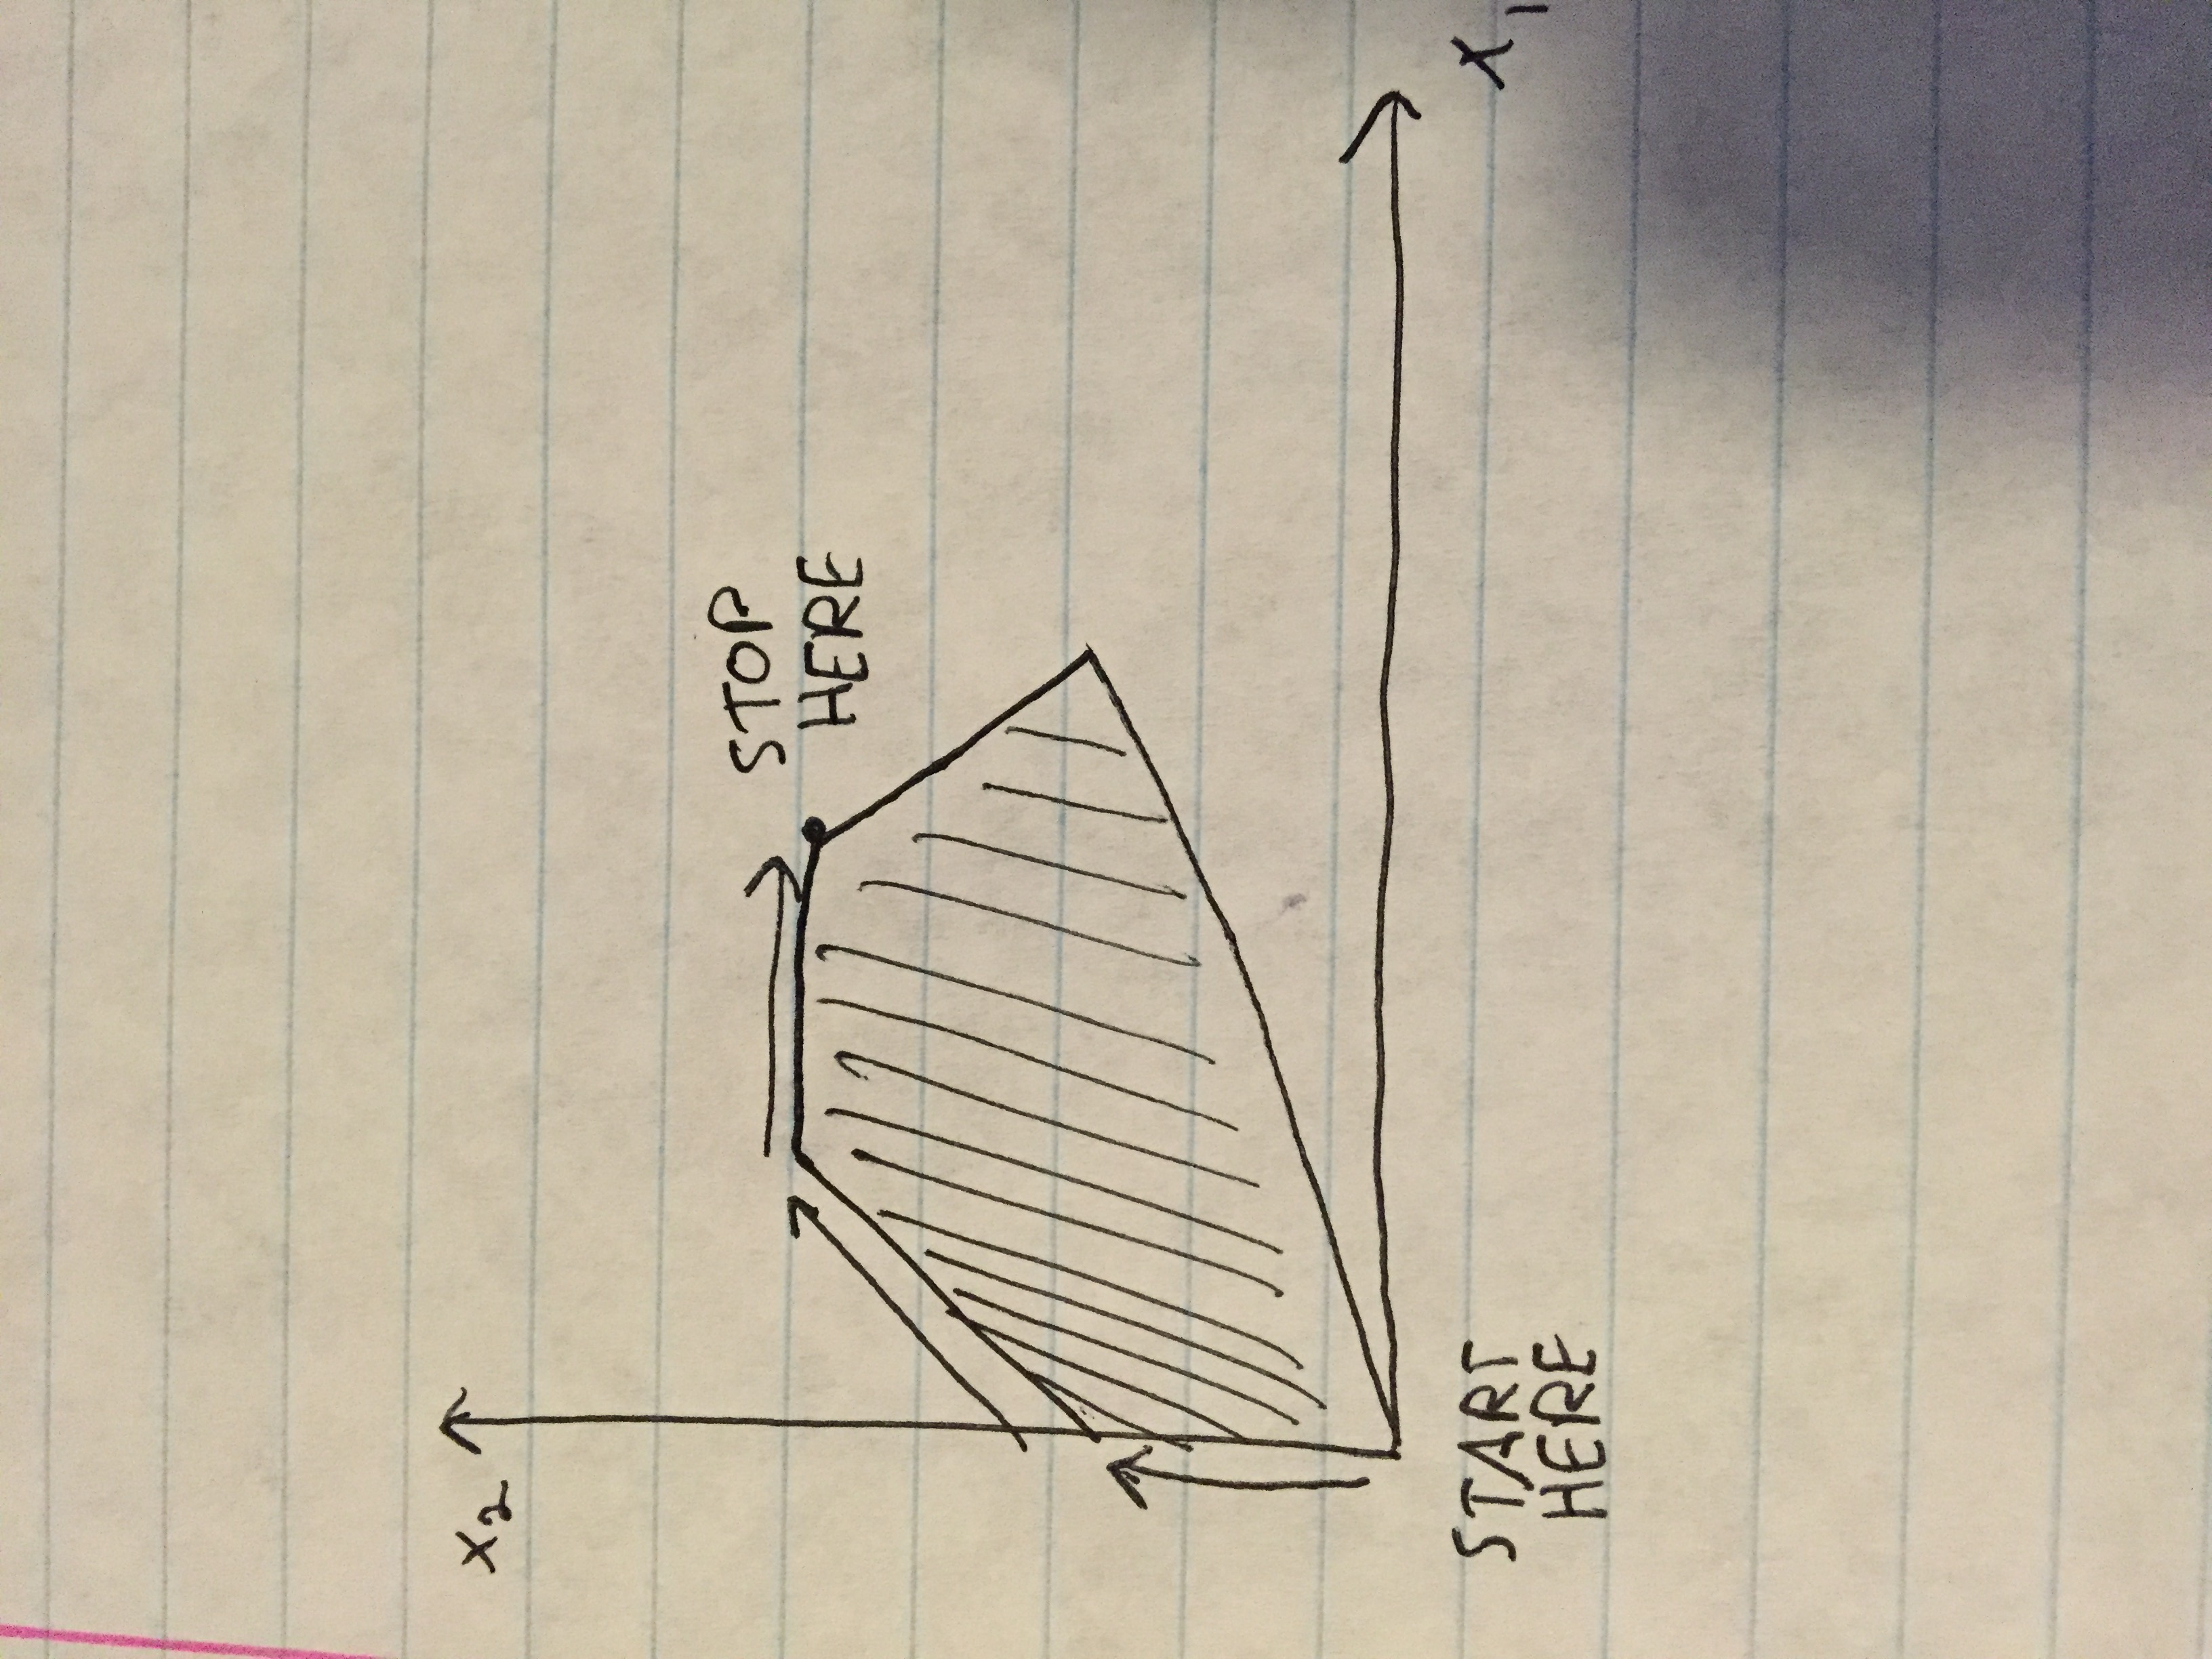
\includegraphics[width=\linewidth,angle=-90]{simplex.jpg}
    \caption{Path of Simplex algorithm}
  \end{figure}
\end{enumerate}
\end{document}
